\documentclass[times,specification,annotation]{itmo-student-thesis}

%% Опции пакета:
%% - specification - если есть, генерируется задание, иначе не генерируется
%% - annotation - если есть, генерируется аннотация, иначе не генерируется
%% - times - делает все шрифтом Times New Roman, собирается с помощью xelatex
%% - languages={...} - устанавливает перечень используемых языков. По умолчанию это {english,russian}.
%%                     Последний из языков определяет текст основного документа.

%% Делает запятую в формулах более интеллектуальной, например:
%% $1,5x$ будет читаться как полтора икса, а не один запятая пять иксов.
%% Однако если написать $1, 5x$, то все будет как прежде.
\usepackage{icomma}

%% Один из пакетов, позволяющий делать таблицы на всю ширину текста.
\usepackage{tabularx}

%% Данные пакеты необязательны к использованию в бакалаврских/магистерских
%% Они нужны для иллюстративных целей
%% Начало
\usepackage{tikz}
\usetikzlibrary{arrows}
\usepackage{filecontents}
\begin{filecontents}{bachelor-thesis.bib}
@online{ graph-attention-networks,
    year        = {2018},
    title       = {Graph Attention Networks},
    author      = {\colorbox{orange}{имена не на английском}},
    url         = {https://arxiv.org/abs/1710.10903},
    year        = {2018},
    langid      = {english}
}

@online{ gated-graphs-nn,
    year        = {2018},
    title       = {Learning to Represent Programs with Graphs},
    author      = {Miltiadis Allamanis, Marc Brockschmidt, Mahmoud Khademi},
    url         = {https://arxiv.org/abs/1711.00740},
    year        = {2018},
    langid      = {english}
}

@online{ tree-gen,
    year        = {2019},
    title       = {TreeGen: A Tree-Based Transformer Architecture for Code Generation},
    author      = {Zeyu Sun, Qihao Zhu, Yingfei Xiong},
    url         = {https://arxiv.org/abs/1911.09983},
    year        = {2019},
    langid      = {english}
}

@online{ code2vec,
    year        = {2019},
    title       = {code2vec: Learning Distributed Representations of Code},
    author      = {Uri Alon, Meital Zilberstein, Omer Levy},
    url         = {https://arxiv.org/abs/1803.09473},
    year        = {2019},
    langid      = {english}
}

@online{ slm,
    year        = {2019},
    title       = {Structural Language Models of Code},
    author      = {Uri Alon, Roy Sadaka, Omer Levy},
    url         = {https://arxiv.org/abs/1910.00577},
    year        = {2020},
    langid      = {english}
}

@inproceedings{ example-english,
    year        = {2015},
    booktitle   = {Proceedings of IEEE Congress on Evolutionary Computation},
    author      = {Maxim Buzdalov and Anatoly Shalyto},
    title       = {Hard Test Generation for Augmenting Path Maximum Flow 
                   Algorithms using Genetic Algorithms: Revisited},
    pages       = {2121-2128},
    langid      = {english}
}

@article{ example-russian,
    author      = {Максим Викторович Буздалов},
    title       = {Генерация тестов для олимпиадных задач по программированию 
                   с использованием генетических алгоритмов},
    journal     = {Научно-технический вестник {СПбГУ} {ИТМО}},
    number      = {2(72)},
    year        = {2011},
    pages       = {72-77},
    langid      = {russian}
}

@article{ unrestricted-jump-evco,
    author      = {Maxim Buzdalov and Benjamin Doerr and Mikhail Kever},
    title       = {The Unrestricted Black-Box Complexity of Jump Functions},
    journal     = {Evolutionary Computation},
    year        = {2016},
    note        = {Accepted for publication},
    langid      = {english}
}

@book{ bellman,
    author      = {R. E. Bellman},
    title       = {Dynamic Programming},
    address     = {Princeton, NJ},
    publisher   = {Princeton University Press},
    numpages    = {342},
    pagetotal   = {342},
    year        = {1957},
    langid      = {english}
}
\end{filecontents}
%% Конец

%% Указываем файл с библиографией.
\addbibresource{bachelor-thesis.bib}

\begin{document}

\studygroup{M3436}
\title{Генерация Kotlin кода с помощью нейронной сети архитектуры Transformer для фаззинга компилятора}
\author{Тихонов Виталий Андреевич}{Тихонов В.А.}
\supervisor{Фильченков Андрей Александрович}{Фильченков А.А.}{канд. физ.-мат. наук}{доцент, научный сотрудник Университета ИТМО}
\publishyear{2021}
%% Дата выдачи задания. Можно не указывать, тогда надо будет заполнить от руки.
\startdate{01}{сентября}{2020}
%% Срок сдачи студентом работы. Можно не указывать, тогда надо будет заполнить от руки.
\finishdate{31}{мая}{2021}
%% Дата защиты. Можно не указывать, тогда надо будет заполнить от руки.
\defencedate{\colorbox{orange}{15}}{июня}{2021}

\addconsultant{Петухов В.А.}{без степени, без звания}

\secretary{Павлова О.Н.}

%% Задание
%%% Техническое задание и исходные данные к работе
\technicalspec{Требуется попробовать применить нейронные сети, построенные на архитектуре
Transformer для генерации кода на языке Kotlin. В архитектуру сети должна быть заложена
генерация кода не только в соответствии с грамматикой языка (правила синтаксиса), но и в
соответствие с некоторыми правилами семантики.}

%%% Содержание выпускной квалификационной работы (перечень подлежащих разработке вопросов)
\plannedcontents{\begin{enumerate}
    \item Провести обзор существующих архитектур нейронных сетей Transformer и сделать
аргументированный выбор трансформера для генерации кода.
    \item Изучить существующие способы делать code embedding и выбрать наиболее подходящий
для решаемой задачи.
    \item Обучить сеть на наборе тестов компилятора и/или фрагментов кода в багтрекере.
    \item Применить построенный генератор кода для поиска проблем в компиляторе Kotlin:
выбрасываемых исключений и проблем с производительностью.
\end{enumerate}}

%%% Исходные материалы и пособия 
\plannedsources{Исходные материалы и пособия работой не предусмотрены}

%%% Цель исследования
\researchaim{Разработать модель поддерживающую обучение элементам семантики языка для более качественной генерации кода}

%%% Задачи, решаемые в ВКР
\researchtargets{\begin{enumerate}
    \item Реализовать модель для генерации кода
    \item Раширить модель, поддержав обработку некоторой семантичекой информации
    \item Оценить пользу от добавления семантичекой информации
    \item Использовать модель для генерации кода и выявления проблем компилятора
\end{enumerate}}

%%% Использование современных пакетов компьютерных программ и технологий
\addadvancedsoftware{IntelliJ IDEA}{2, 3}
\addadvancedsoftware{PyCharm}{2, 3}
\addadvancedsoftware{Google Colab}{3}

%%% Краткая характеристика полученных результатов 
\researchsummary{\colorbox{orange}{На данный момент результатов получено не было}}

%%% Гранты, полученные при выполнении работы 
\researchfunding{нет}

%%% Наличие публикаций и выступлений на конференциях по теме выпускной работы
\researchpublications{нет}

%% Эта команда генерирует титульный лист и аннотацию.
\maketitle{Бакалавр}

%% Оглавление
\tableofcontents

%% Макрос для введения. Совместим со старым стилевиком.
\startprefacepage

Процесс тестирования очень важен при разработке приложений. Причина в том, что продукт, работающий некачественно может доставлять пользователям дискомфорт, приводить к потере времени и денег, а это в свою очередь может стать поводом для отказа от продукта. Еще важнее тестировать приложения, не являющиеся конечным продуктом, ведь проблемы в них могут затронуть еще большее число пользователей. Одним из таких приложений являются компиляторы языков программирования.

Классический подход в разработке тестов - написание тестов программистами, сразу после обновления функционала программы. Очевидно, что таким способом сложно протестировать настолько большую программу как компилятор достаточно хорошо, поэтому необходимы и другие методы тестирования.

Примером такого метода может быть фаззинг. В процессе фаззинга для тестируемой программы генерируется большое количество экземпляров входных данных. Для каждого примера входных данных программа запускается независимо, и исследуются некоторые характеристики ее работы, такие, например, как затрачиваемые память и время. Входные данные на которых поведение программы аномально (например, фиксируется большое количество затраченной памяти или долгое время работы) выделяются для дальнейшего изучения программистом.

В данной работе в качестве тестируемого приложения выбран компилятор языка Kotlin. В случае с фаззингом компитлятора в качестве входных данных будут использоваться программы, написанные на соответствующем языке, а критериями аномальности могут служить время компиляции, затраченная память, выброшенные исключения, отличающееся поведение откомпилированных входных программ на разных платформах или разных версиях компилятора.

Получается, что в данном случае задача тестирования сводится к задаче генерации кода. Есть два основных аспекта, которые следует учитывать при генерации кода - это синтаксис и семантика языка. С синтаксисом языка программирования не должно возникать серьезных проблем - он описывается формальной грамматикой, и нет трудностей в генерации кода на ее основе. С семантикой все сложнее - у нее нет формального описания. В случае Kotlin'а она описывается спецификацией на естественном языке. Реализовать генератор, полностью поддерживающий спецификацию - задача сопоставимая с разработкой самого компилятора. Более того, генератор будет иметь неформальную основу, а значит высоки шансы допустить ошибки при его разработке.

При этом опираться только на синтаксис нельзя - доля семантически некорректных, а значит некомпилируемых программ слишком высока. Поэтому возникает желание изучить семантику с помощью машинного обучения, вместо того чтобы формализовывать ее или писать сложный генератор, описывая всю спецификацию. Однако современные решения почти не предусматривают непосредственную передачу модели семантической информации в качестве входных данных.

Таким образом формулируется цель работы - разработать модель нейронной сети, обучаемую семантике языка Kotlin для генерации корректного кода для фаззинга компилятора.

В первой главе описываются некоторые существующие подходы к извлечению информации из исходного кода, выбирается базовый подход для дальнейшего улучшения. Во второй главе рассмативаются возможные улучшения базового подхода за счет добавления информации о семантике. Заключительная третья глава рассказывает о процессе реализации, проблемах, возникших на этом этапе и их устранении.


%% Начало содержательной части.
\chapter{Обзор существующих решений}

Для начала необходимо разобраться разобраться как работать с такими сложными данными как исходный код. 
Модели машинного обучения отлично умеют работать с числами. Однако работать напрямую с текствой информацией они не могут. Тут на помощь приходит механизм эмбедингов - данные разбиваются на структурные компоненты (например, текст можно разбить на слова, а исходный код на токены), и каждой такой компоненте сопостовляется вектор чисел, называемый эмбедингом. Таким образом каждый элемент кодируется точкой в некотором пространстве. Обработанные таким образом данные уже можно подавать на вход модели.

Существуют способы предлагать эти вектора по-умному, сохраняя некоторую семантическую информацию. Например, может получиться так, что вектор между точками, соответствующим словам "Москва" и "Россия" будет коллинеарен аналогичному вектору для слов "Прага" и "Чехия". То есть такой вектор будет иметь смысл "x является столицей y".

Текст имеет достаточно простую структуру - это по сути просто последовательность слов. Для работы с последовательностями существуют рекуррентные нейронные сети, принимающие данные фармент за фрагментом. Исходный же код имеет более сложную древовидную структуру. Это приводит к некоторым интересным спецэффектам. Например, на уровне файла мы можем поменять местами определеня двух функций, и код от этого никак не изменится. Однако, если в тексте поменять местами два абзаца, то смысл может значительно поменяться. Другим примером являются многозначные слова. В случае с Java это может быть слово \texttt{final} или \texttt{static}, имеющие разные значения в зависимости от контекста, а конструкция \texttt{String s} может быть как объявлением переменной, так и параметром функции. В Kotlin'е есть ключевые слова \texttt{get}, \texttt{set}, \texttt{field}, которые в то же время могут использоваться как идентификаторы. Выходит, что рассматривать код как обычный текст - не лучшая затея, так как часть информации из входных данных просто не будет использоваться.

Другое хорошо изученное представление данных - изображения. Для работы с ними так есть целый класс нейронных сетей - сверточные. Изображения рассматриваются как двумерные объекты, полностью заполняя некоторый прямоугольник.

Графовое предствление данных находится где-то по середине, не умещаясь в одномерное пространство, при этом не заполняя полностью двумерное. Поэтому для графов как правило используются специальные подходы.

\section{Способы обработки кода}\label{workingWithCode}
Код можно рассматривать в некотором смысле как текст, а значит модели машинного обучения не смогут работать с ним напрямую. Поэтому необходимо разобраться в подходах, позволяющих представлять исходный код в виде векторов. Рассмотрим подробнее несколько подходов по представлению исходного кода и выберем наиболее подходящий для генерации кода.

\subsection{Тривиальные подходы}\label{trivial}
Наиболее очевидным подходом к извлечению информации из кода являются разбение исходного кода программы на токены и обучение модели, основанной на рекуррентной сети на полученной последовательности. Как было сказано ранее, в таком случае часть информации утрачивается и не учитывается моделью.

Более разумным будет построение дерево разбора для исходного кода. Деревья разбора содержат гораздо больше полезной информации, чем код, представленный в виде текста. Например, если код из листинга~\ref{lst1} рассматривать последовательно, то мы поймем, что есть некоторый класс \texttt{A}, с которым ассоциируются поля \texttt{x: Int} и \texttt{y: Int}. При этом дерево разбора этого фрагмента, изображенное на рисунке~\ref{deep} слева имеет более сложную структуру: тут явно указано, что \texttt{x: Int} относится к конструктору класса.

\begin{lstlisting}[float=!h,caption={Пример исходного кода на Kotlin},label={lst1}]
class A(val x: Int) {
    val y: Int = 10
}
\end{lstlisting}

Чтобы модель могла работать с деревом предлагается обучить эмбединги для каждого типа вершин, а само дерево представять как последовательность вершин в порядке обхода в глубину. Полученную последовательность можно отдавать на вход модели на основе рекуррентной сети. Для графа, изображенного справа на рисунке~\ref{deep} обход в глубину будет выгляеть следующим образом: $P$, $A$, $B$, $D$, $E$, $F$, $C$. Но не смотря на то что самом графе расстояние между вершинами $B$ и $C$ равно двум, в полученной последовательности путь значительно вырос и равен четырем. Для решения такой проблемы можно добавить в путь стрелку вверх, если делается подъем, и стрелку вниз, если делается спуск. В таком случае результат обхода будет следующим: $P$, $\downarrow$, $A$, $\downarrow$, $B$, $\downarrow$, $D$, $\downarrow$, $E$, $\downarrow$, $F$, $\uparrow$, $\uparrow$, $\uparrow$, $\uparrow$, $\downarrow$, $C$. Стрелки - специальные символы, для которых также обучаются эмбединги.

\begin{figure}[!h]
    \caption{Слева AST для листинга~\ref{lst1}, справа - пример дерева}\label{deep}
    \centering
    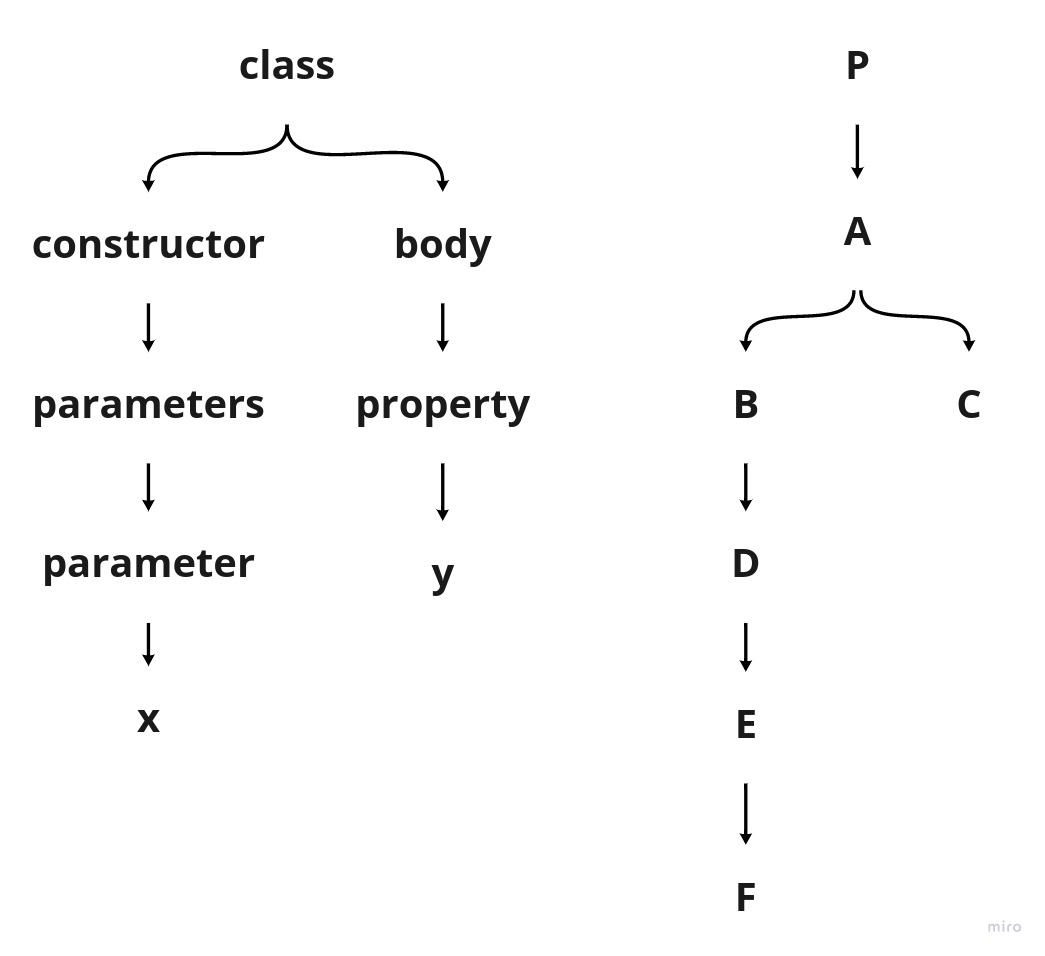
\includegraphics[width=0.6\textwidth]{deep.jpg}
\end{figure}

\subsection{Графовые нейронные сети}\label{sec:gnn}
Значительно более мощным является подход с использованием графовых нейронных сетей (Graph Neural Network - GNN). Каждой вершине сопостовляется вектор состояния, после чего происходит несколько этапов обмена информации между вершинами. Этап состоит из двух фаз: отправка сообщений и получение сообщений. Во время первой фазы для каждой вершины вычисляется сообщение для отправки. В качестве сообщения используется вектор состояния, преобразованный каким-либо образом. После того как все сообщения вычислины, вершины передают сообщения своим соседям, начинается вторая фаза. Во время фазы получения сообщений каждая вершина агрегирует получаемые от других вершин сообщения, например, в работе~\cite{graph-attention-networks} сообщения взвешенно усреднются с использованием механизма внимания. Состояние вершины обновлятеся с помощью полученного только что агрегированного сообщения. Это можно сделать, например, с помощью конкетенации этих векторов и линейного предобразования для уменьшения размерности конкатенированного вектора до исходной размерности состояния вершины.

Простой вариант - использовать AST в качестве графа. Однако в статье~\cite{gated-graphs-nn} предлагается дополнить этот граф ребрами data-flow графа. Например, можно соеденить вызов функции и возвращаемое значение из опредленение функции или аргументы вызова с параметрами функции. В таком случае информация по графовой нейронной сети в некоторых случаях будет передаваться также как и в исходном коде.

\subsection{Дерево разбора как список правил}\label{sec:treegen}
Дерево разбора можно представить в виде последовательности, но значительно хитрее, чем в описанном ранее случае, где дерево заменялось на список вершин в порядке обхода в глубину. Подход, используемый в статье~\cite{tree-gen} рассматривает синтаксическое дерево как последовательность приминения правил грамматики.

\begin{figure}[!h]
    \caption{Слева некоторые правила грамматики, справа - дерево, получающееся при последовательном применении правил 1, 7, 12, 20}\label{treegen}
    \centering
    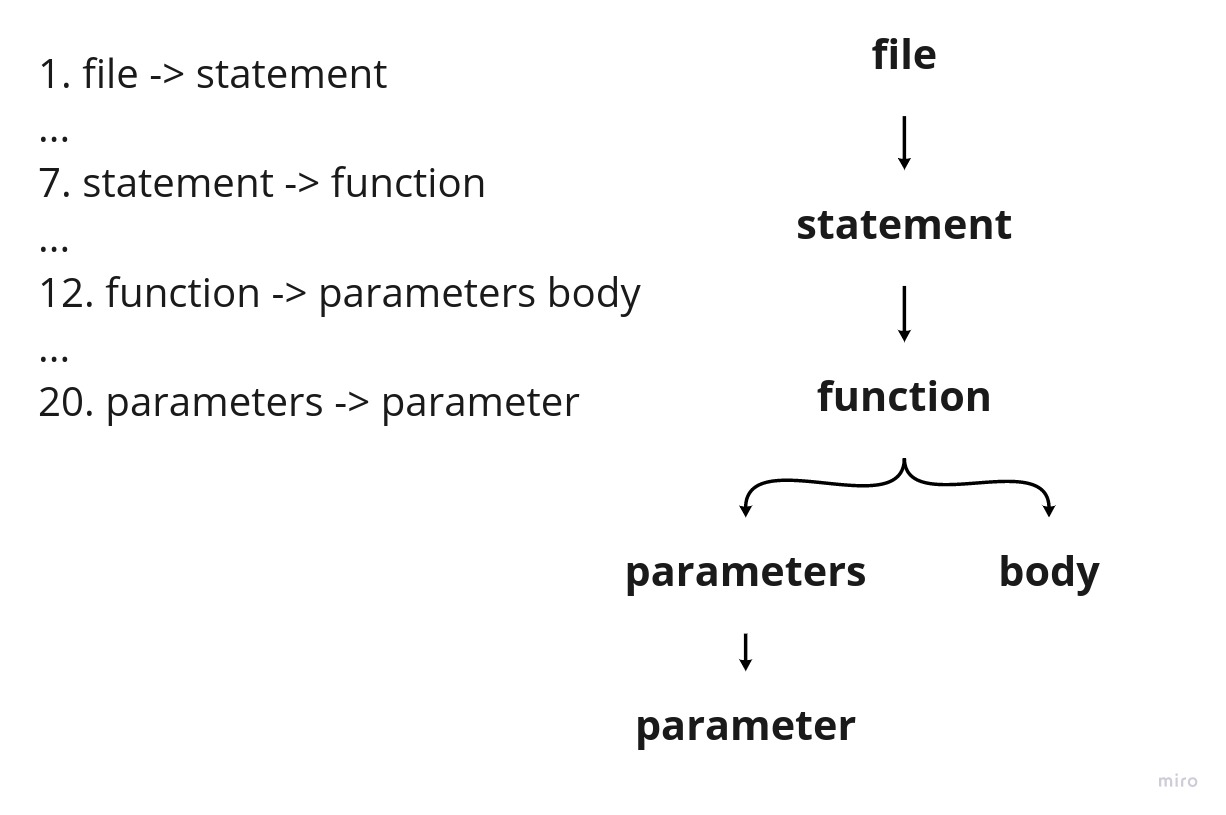
\includegraphics[width=0.7\textwidth]{treegen.jpg}
\end{figure}

Рассмотрим пример. Слева на рисунке~\cite{treegen} указаны некоторые правила грамматики. Будем считать, что \texttt{file} - это стартовый нетерминал, тогда после использования правил 1, 7, 12, 20 дерево примет вид изображенный справа на том же рисунке. В качестве текущего нетерминала для раскрытия выбирается первый в порядке обхода в глубину. То есть следующее правило будет раскрывать нетерминал \texttt{parameter}. Такое решение описывает исходный код очень близко к грамматике.

\subsection{Дерево разбора как набор путей}\label{sec:slm}
Еще один подход для представления дерева разбора кода рассмотрен в статье~\cite{code2vec}. При таком способе AST представляется в виде набора путей между всеми парами вершин в дереве. Далее эбмединги путей проходят через блок трансформера, механизм внимания позволяет выделить наиболее важные пути, после чего они взвешенно суммируются. Таким образом вычислятеся векторное представление примера кода.

Логику этого подхода продолжает статья~\cite{slm}. Там ставится задача предсказания вершины по контексту (code completion). В качестве входных данных на очередном шаге используются пути от всех листьев до родителя предсказываемой вершины, а также путь от корня дерева. \colorbox{orange}{пример, в том числе с несколькими предсказаниями}

\subsection{Выбор модели}\label{sec:chooseModel}
Для задачи генерации кода графовые нейронные сети не самый лучший вариант. Во-первых, не приминялись \colorbox{orange}{??}. Во-вторых, они тяжело учатся \colorbox{orange}{??}.

Подход со списком правил выглядит неплохим вариантом, но \colorbox{orange}{что?))) Наверное можно сказать что он постарее, чем SLM и нигде??? больше не применялся}. Тем не менее его можно рассмотреть в дальнейших исследованиях.

В данной работе в качестве основы выбран подход из статьи \colorbox{orange}{Structural} language models of code. В целом подход себя зарекомендовал для решения таких задач как предсказание имени метода и \colorbox{orange}{возможно для чего-то еще}. Более того, конкретно в этой статье подход используется для генерации (пусть и небольших фрагментов) кода.

\colorbox{orange}{надо чета сказать про трансформеры}

\section{Подходы к извлечению семантической информации}\label{sec:semantic}
\colorbox{orange}{налить воды}
\subsection{Предсказание типов}\label{sec:lambdanet}
LambdaNet?

\subsection{Семантические ребра}\label{sec:semanticEdges}
семантические ребра из ggnn

\section{Улучшение модели}\label{sec:improve}
Практически во всех указанных работах модели не используют напрямую семантическую информацию. Исключением является статья \colorbox{orange}{GGNN}, где внедряют информацию о типах \colorbox{orange}{каких именно}, пытаясь обучить решетку на типах. Такой подход позволяет частично сохранить иерархию типов, даже для новых, не видимых на этапе обучения типов. Однако типы определяются не только иерархией. Кроме нее, есть как минимум поля и методы, которые можно вызвать на экземпляре класса.

Поэтому ставится задача внедрить механизмы работы с семантикой в модель

\chapterconclusion
вфвф


\chapter{Обработка семантики}

Во второй главе исследовательской работы описывается:
Предлагаемое теоретическое решение (подход/метод/алгоритм/схема)
Обоснование, почему оно удовлетворяет требованиям, сформулированным в первой главе.
Теоретическое сравнение с существующими решениями

\section{Добавление семантики}\label{addSemantic}

\subsection{Типы}\label{sec:types}

Подход для эмбедингов типов

\subsection{Семантические токены}\label{sec:tokens}

обрезка путей на невидимой информации?? (private)

\chapterconclusion

В конце каждой главы желательно делать выводы. Вывод по данной главе~--- нумерация работает корректно, ура!


\chapter{Реализация}

\section{Имплементация модели}\label{sec:impl}
Имплементация модели

\section{Извлечение путей}\label{sec:extract}
Фильтрация датасета, afterLastTree, выбор глубины

\section{Архитектура генератора}\label{sec:generator}
Архитектура генератора (в том числе ограничение на длину и ширину)

\section{Интеграция сематники}\label{sec:semanticIntegration}
Интеграция сематники

\section{Результаты генерации}\label{sec:generationResult}
Результаты генерации

\chapterconclusion
фывфв


%% Макрос для заключения. Совместим со старым стилевиком.
\startconclusionpage

В данном разделе размещается заключение.

\printmainbibliography

\end{document}

